\chapter{Descripción del problema} \label{cap:capitulo2}

El objetivo de este trabajo es plantear e implementar una solución que permita calcular la frecuencia media de nado de un nadador a partir de una secuencia de vídeo. En el presente capítulo se presentan los requisitos y detalles del problema, un análisis de los trabajos que ya se han llevado a cabo en este ámbito y una breve introducción del método propuesto. Finalmente, se detalla el sistema de captación con el que se han grabado los vídeos que utilizaremos.

Para comenzar, definimos la frecuencia media de nado como el número de brazadas que realiza un nadador por unidad de tiempo o el número de brazadas que han sido necesarias para avanzar una cierta distancia. A su vez, podríamos definir brazada como el movimiento enérgico que se hace extendiendo y recogiendo ambos brazos y que permite generar el impulso suficiente para que el nadador avance por el agua de la piscina.  

En las competiciones de natación, los diferentes nadadores deben recorrer un determinado número de veces el largo de la piscina, el cual suele recibir el nombre de ``split''. La piscina de la Facultad de Ciencias del Deporte de la UGR tiene un largo de 25 metros, al ser una piscina semi-olímpica. 

Queremos calcular el número de brazadas que un determinado nadador realiza en cada uno de los splits. Para ello, se nos indica que deberemos despreciar la distancia recorrida gracias al salto del nadador desde el trampolín y la voltereta con la que se cambia el sentido del nado. Estos instantes no son de interés dado que el nadador no bracea de forma continuas, si no que utiliza el impulso del salto y la propulsión con la pared, respectivamente. También queremos calcular el número de brazadas por minuto a lo largo de toda la prueba, con las mismas consideraciones que se acaban de mencionar.

\section{Trabajos relacionados}

La especificación de sistemas que calculen de forma automática la frecuencia de nado ya ha sido abordada en el pasado. Sin embargo, la mayoría de artículos consultados, como \cite{swimmerautostrokeratio}, hacen uso de sensores adheridos al cuerpo o traje de baño del nadador con tal fin, en lugar de secuencias de vídeo.

Aquellos trabajos que hacen uso de secuencias de vídeo se centran en la detección del nadador, y valoran el uso de diversas técnicas con dicho fin.

Trabajos como \cite{swimmerarti} proponen el uso del espacio de color HSV (Hue, Saturation, Value) y el uso del algoritmo de sustracción de fondos MOG (Mixture of Gaussians) para diferenciar zonas en movimiento de zonas estáticas. Posteriormente, se utiliza el método \textit{Mean Shift Clustering} para delimitar el contorno del nadador. Estos datos se utilizan para entrenar a un detector capaz de seguir el movimiento del nadador a lo largo de la piscina. En el artículo se hace especial hincapié en la dificultad de la detección del nadador debido a los cambios en el ambiente que produce el chapoteo en el agua y los reflejos en el agua de las fuentes de luz.

Otras investigaciones, como \cite{swimmerartii}, prestan especial atención a la influencia del espacio de color utilizado. Tras analizar el rendimiento del método de Yoon \cite{yoonmethod} sobre el espacio de color RGB (Red, Green, Blue) y la aplicación del algoritmo MOG sobre la representación HSV, como en \cite{swimmerarti}, el autor propone un método para detectar nadadores basado en las diferencias de los valores de las bandas de crominancia del espacio de color YCbCr.

En otros artículos se deja de lado el uso de técnicas clásicas del procesamiento de imágenes y se propone el uso de redes neuronales para detectar a los nadadores. Trabajos como \cite{swimmerartiv} utilizan redes neuronales para distinguir si el nadador está saltando desde el trampolín, nadando, buceando, o cambiado el sentido del nado. Otros, como \cite{swimmerartvi}, utilizan la inteligencia artificial para detectar las distintas posiciones en las que se puede encontrar un nadador durante una carrera. A partir de la sucesión de estas etapas se calcula la frecuencia de nado. En \cite{swimmerartiii} se discute el rendimiento de diversos tipos de redes neuronales convolucionales entrenadas para distinguir si un nadador está realizando una brazada o no. La frecuencia de nado se calcula a partir del número de detecciones que realice la red neuronal por unidad de tiempo. 

Cabe mencionar que también existen investigaciones \cite{swimmerartv} que utilizan técnicas de procesamiento de histogramas para detectar al nadador y seguir su movimiento.

La mayoría de trabajos consultados se centran solamente en la detección del nadador, o en la identificación de las diversas etapas por las que pasa un nadador en una carrera, sin calcular su frecuencia media de nado, objetivo último de este trabajo. Solamente \cite{swimmerartiii} y \cite{swimmerartvi} prestan atención a este aspecto. Como mencionamos anteriormente, en \cite{swimmerartvi} se utiliza la sucesión entre las etapas que conlleva una brazada, detectadas por una red neuronal, para calcular cuando el nadador está braceando y por consiguiente su frecuencia de nado, mientras que en \cite{swimmerartiii} se utiliza las detecciones de una red neuronal entrenada para detectar momentos en los que el nadador se encuentra realizando la brazada para posteriormente calcular la frecuencia de nado.

También cabe mencionar que existen compañías que ofrecen sistemas de cámaras y paquetes software, como \textit{\href{https://www.swimmingcam.com/}{Swimpro}} y \textit{\href{https://www.dartfish.com/swimming}{Dartfish}}, con los que obtener diversas métricas sobre el rendimiento de los nadadores, entre las que se encuentran la frecuencia media de nado. Sin embargo, y como era de esperar, estas compañías no ofrecen información alguna sobre cómo realizan sus cálculos.

Dado que el material del que partimos es significativamente diferente al usado por la mayoría de artículos, proponemos un modelo propio para calcular la frecuencia media de nado. 

\section{Método propuesto}

El método que proponemos en este trabajo tiene dos pasos diferenciados: (i) detección del nadador y (ii) estimación de brazadas.

En primer lugar, necesitamos poder reconocer al nadador durante la prueba y estimar la posición de la piscina en la que se encuentra. Tras haber consultado los trabajos previos expuestos anteriormente, decidimos abordar (i) desde dos puntos de vista distintos.

En el capítulo \ref{cap:capitulo3} se propondrá un modelo basado en técnicas clásicas del procesamiento de imágenes. Este buscará distinguir elementos estáticos y dinámicos, y, una vez reconocidos los elementos dinámicos, extraerá el contorno del nadador. En el capítulo \ref{cap:capitulo4} se propondrá un modelo basado en técnicas de aprendizaje profundo para reconocer y ubicar al nadador. 

En la figura \ref{fig:primerejemplodeteccion} se puede apreciar cómo estos métodos nos devuelven una caja que contiene al nadador. Esta nos proporcionará los datos que utilizaremos para el segundo paso: estimar el número de brazadas y calcular la frecuencia media de nado. 

\begin{figure}
    \centering
    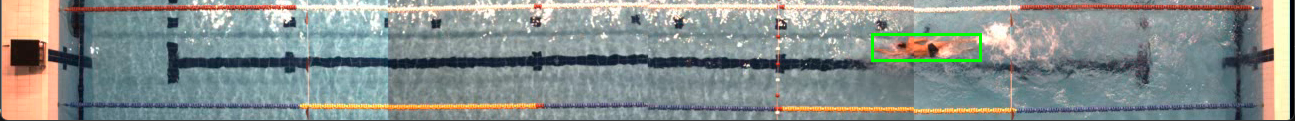
\includegraphics[width=\textwidth,height=\textheight,keepaspectratio]{imagenes/capitulo2/ejemplo_bbox.png}
    \caption{Ejemplo de detección de un nadador.}
    \label{fig:primerejemplodeteccion}
\end{figure}

En la figura \ref{fig:primerejemplovariacionanchura} se puede observar cómo varía la anchura de la caja que contiene al nadador. Dado que el movimiento del nadador tiene un carácter periódico, podemos estimar el número de brazadas (ii) a partir de la variación en la anchura de la caja. Podemos considerar que la brazada se completa en producen en momentos de máxima anchura, ya que el nadador debe extender los brazos. De esta forma, podemos detectar las brazadas de una manera sencilla identificando los máximos de la función.

\begin{figure}[h!]
    \centering
    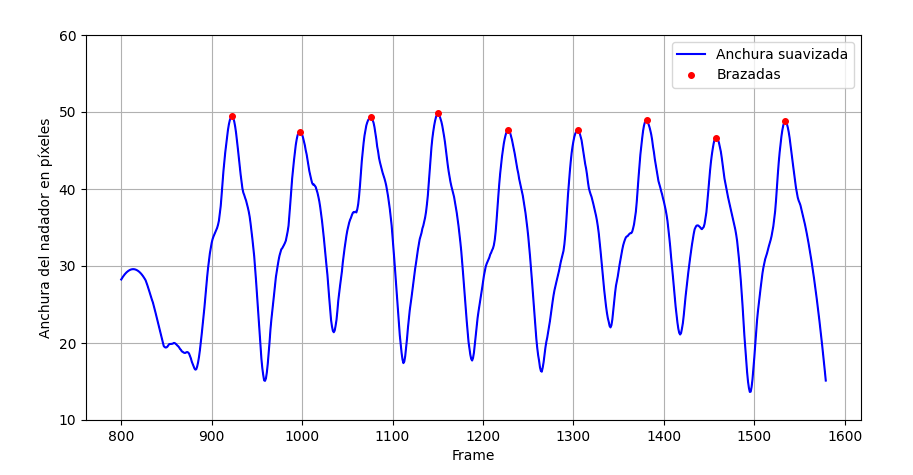
\includegraphics[width=\textwidth,height=\textheight,keepaspectratio]{imagenes/capitulo2/ejemplo_variacion_altura.png}
    \caption{Variación de anchura de la caja que contiene al nadador.}
    \label{fig:primerejemplovariacionanchura}
\end{figure}

Para calcular el tiempo que el nadador tarda en completar un tramo de 25 metros, podemos usar la variación en las coordenadas X de la caja. Estos valores pasarán de tener una tendencia creciente a decreciente, o viceversa, cuando se cambie el sentido del nado. En la figura \ref{fig:primerejemplovariacionsentido} se puede apreciar este hecho. Conocido el número de fotogramas en los que se mantiene cada una de las tendencias, y la tasa de fotogramas por segundo del vídeo, se puede calcular fácilmente el tiempo que se tarda en recorrer cada split.

\begin{figure}[h!]
    \centering
    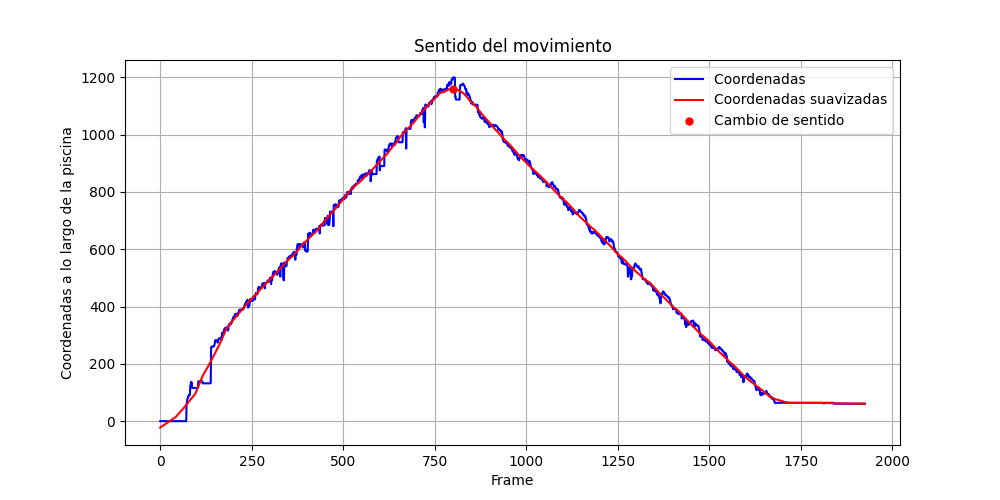
\includegraphics[width=\textwidth,height=\textheight,keepaspectratio]{imagenes/capitulo2/ejemplo_cambio_sentido.png}
    \caption{Variación en las coordenadas X de la caja que contiene al nadador.}
    \label{fig:primerejemplovariacionsentido}
\end{figure}

Estos cálculos, así como consideraciones adicionales a tener en cuenta, se discutirán a lo largo del capítulo \ref{cap:capitulo5}.

\section{Sistema de captación de vídeo}

El presente trabajo se ha diseñado y probado con grabaciones cenitales de los entrenamientos y competiciones que se realizan en las instalaciones de la UGR. Dada su importancia, analizaremos cómo se generan estos vídeos.

En el techo del pabellón en el que se encuentra la piscina de la Facultad de Ciencias del Deporte de la UGR podemos encontrar un sistema de 8 cámaras IP. Estas cámaras se sincronizan mediante software, generando un único vídeo en el que se puede visualizar la piscina completa.

El vídeo es generado mediante \textit{video stitching} \cite{LYU201955}. Esta técnica nos permite generar un único fotograma a partir de las zonas comunes, y que se suelen superponer, de los fotogramas generados por cada una de las cámaras del sistema. De esta manera, podemos obtener una imagen con mayor campo de visión. 

En la figura \ref{fig:pisicinaprimerjemeplo} mostramos un fotograma captado por el sistema de cámaras haciendo uso de esta técnica. En dicho fotograma podemos apreciar la diferencia de iluminación de la parte central de la piscina respecto de los extremos, o el desdoblamiento de la corchera en el centro de la piscina en dos. Estos serán aspectos que tendremos que tener en cuenta durante el desarrollo del trabajo.

\begin{figure}
    \centering
    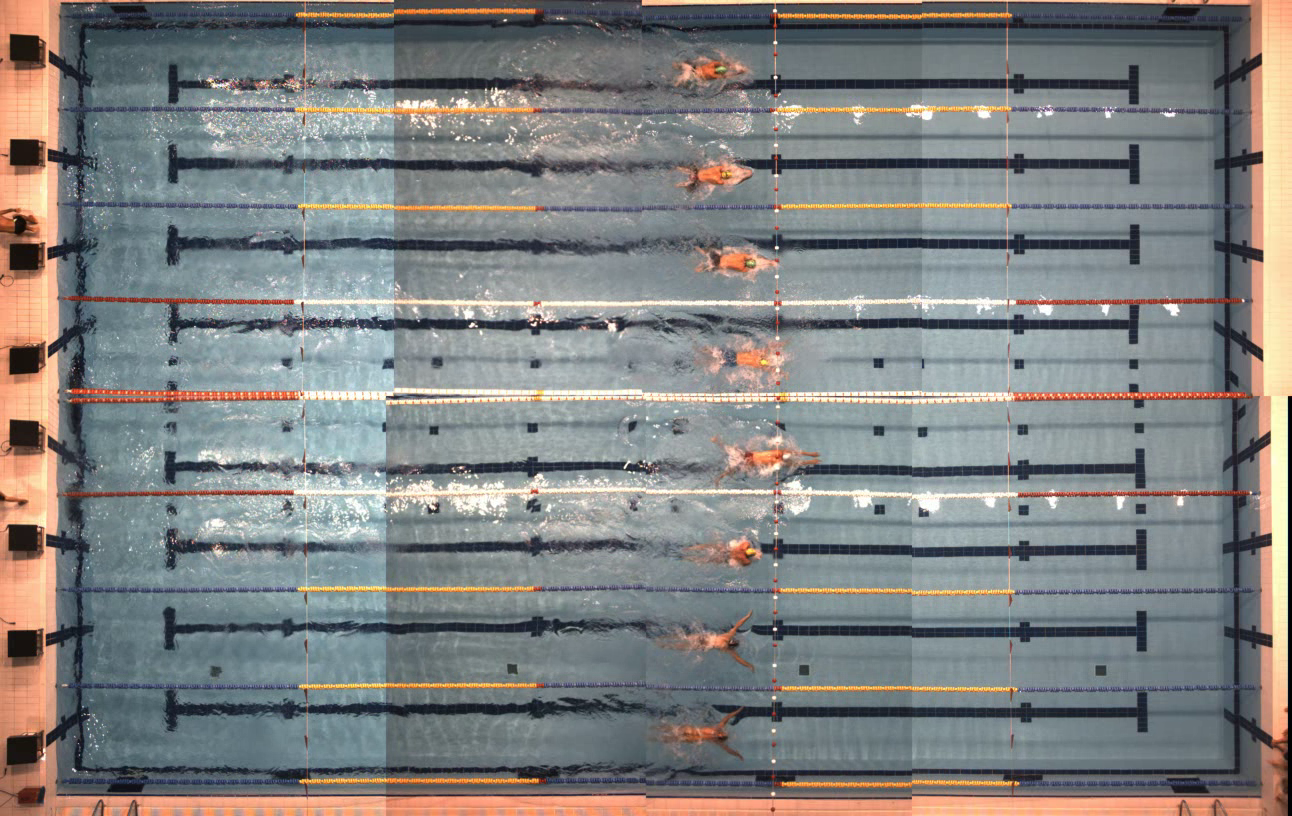
\includegraphics[width=\textwidth,height=\textheight,keepaspectratio]{imagenes/parte_BS/piscina_completa.png}    
    \caption{Fotograma captado por la matriz de cámaras.}
    \label{fig:pisicinaprimerjemeplo}
\end{figure}

Para controlar los parámetros del vídeo generado, tales como resolución y número de fotogramas por segundo, se utiliza el programa \textit{\href{https://www.baslerweb.com/en/products/basler-pylon-camera-software-suite/pylon-viewer/]}{Pylon Viewer}}, el cual también permite capturar imágenes de cada una de las cámaras por separado. La matriz de cámaras instaladas en el pabellón permite grabar a una resolución máxima de 2584x1632 píxeles y una tasa máxima de 83.33 fotogramas por segundo. Sin embargo, normalmente se utiliza una resolución de 1292x816 y una tasa de 41.66 fotogramas por segundo. 

Ahora que se conoce el problema y las características de los vídeos que se utilizarán, se procederá a explicar en detalle cómo se ha llevado a cabo la detección del nadador en los capítulos \ref{cap:capitulo3} y \ref{cap:capitulo4}. El calculo de la frecuencia de nado, a partir de la estimación de las brazadas realizadas por el nadador, se detallará en el capítulo \ref{cap:capitulo5}.

